\chapter{Translation}
\label{ch:translation} % 4000-5000 words

% In this chapter, we describe the overall design of our solution to the problem identified in \Cref{ch:introduction}, building on work described in \Cref{ch:background}.
% TODO: Consider some kind of link from introduction

In this chapter, we discuss the translation process from C++ to Rust of the selected mini-app, HPCCG. First, we introduce the implementation details of HPCCG, along with the translation methodology undertaken. Then, we present a sequence of incrementally performant translations, showing how features of and packages for the Rust language can contribute to the performance of translations of C++ codebases. Next, we discuss approaches for the critical step of program equivalence checking to guarantee comparisons are fair. Finally, we conclude with a section on lessons learned from the process, and a proposed workflow for engineers translating High-Performance C++ codebases to Rust.

% Explain the goals of the effort
The overall goal of this effort is to generate a software product -- a Rust translation of the HPCCG codebase, with strong performance running in serial, and leveraging shared and distributed memory parallelism. On top of this, we propose a approaches for equivalence checking such translations, and use them to give confidence the Rust translation of HPCCG can be used for fair performance comparisons with the reference C++ version.

% Explain the difficulties of the effort
% No-one else has done a whole mini-app, just single kernels and toy examples
As discussed in \Cref{ch:background}, this translation effort is novel with respect to assessing High-Performance Computing for a number of reasons. Previous literature has translated only single computation kernels \cite{} with support for shared and distributed memory parallelism, or very short ``toy example'' applications of around only 150 lines \cite{} \cite{} with support for only shared memory parallelism. In contrast to this, HPCCG is a standard mini-app as part of the Mantevo suite, with the C++ version totalling 1524 lines and having support for both shared and distributed memory parallelism. This order of magnitude increase in codebase length over modern existing work \cite{}, along with support for distributed memory parallelism outside of single computation kernel contexts provides a valuable insight into the suitability of Rust in High-Performance Computing, but at the cost of significant developer effort as compared with existing work.

\section{Design}
\label{sec:translation-design} % 500 words

In traditional software development tasks, such as building the HPC MultiBench tool discussed in \Cref{ch:hpc-multibench}, system design is paramount to building a coherent product. However, for translation tasks the reference implementation has already been designed. As a result of this, the majority of the effort is in understanding the codebase to be translated, and identifying difficulties arising from the differences in program model between the original and target language.

\subsection{Differences in the Rust and C++ programming models}
\label{sec:rust-cpp-programming-models}

Every programming language can be though of as presenting a different abstraction over the capabilities of a variety of physical computer hardware. For low-level languages such as Assembly, this abstraction directly maps to the machine code instructions executed on the bare metal. Above this, languages such as C provide abstractions for common structures such as iteration, but require manual management of properties of the machine such as memory allocation. High-level scripting languages such as Python provide abstractions over memory management as well, leaving an interface very devolved from the hardware it runs on. Across many languages, the problem of program translation is reconciling these abstractions to allow the expression of the original functionality in another language.

Typically, the abstractions across programming languages are equally powerful. However, there are some caveats to this. Lambda Calculus was one of the first expressions of computation within the young field of computer science, proposed by Alonzo Church in 1933 \cite{church1932set}. Seven years later in 1940, Church proposed Simply-Typed Lambda Calculus \cite{church1940formulation}, which restricts the domain of valid programs from all programs to only well-typed ones. This is referred to as a reduction in power of the language. However, this reduction in power is beneficial to programmers, as incorrectly-typed programs are not useful. % todo: explain why/how - can't be run or internally inconsistent?

This restriction of valid programs being well-typed in Simply-Typed Lambda Calculus is mirrored by the prohibition of undefined behaviour in Rust, as shown in Figure \ref{fig:excalidraw_programs_venn}. It is beneficial to programmers, as they largely do not want to write programmers which exhibit on undefined behaviour. This is supported by the fact that programmers in other languages like C++ use dynamic and static analysis tools such as Valgrind \cite{ValgrindHome} and AddressSanitiser \cite{Sanitizers2023} to guarantee these properties outside the compiler

% TODO: Consider replacing this diagram with tikz?
\begin{figure}[H]
    \centering
    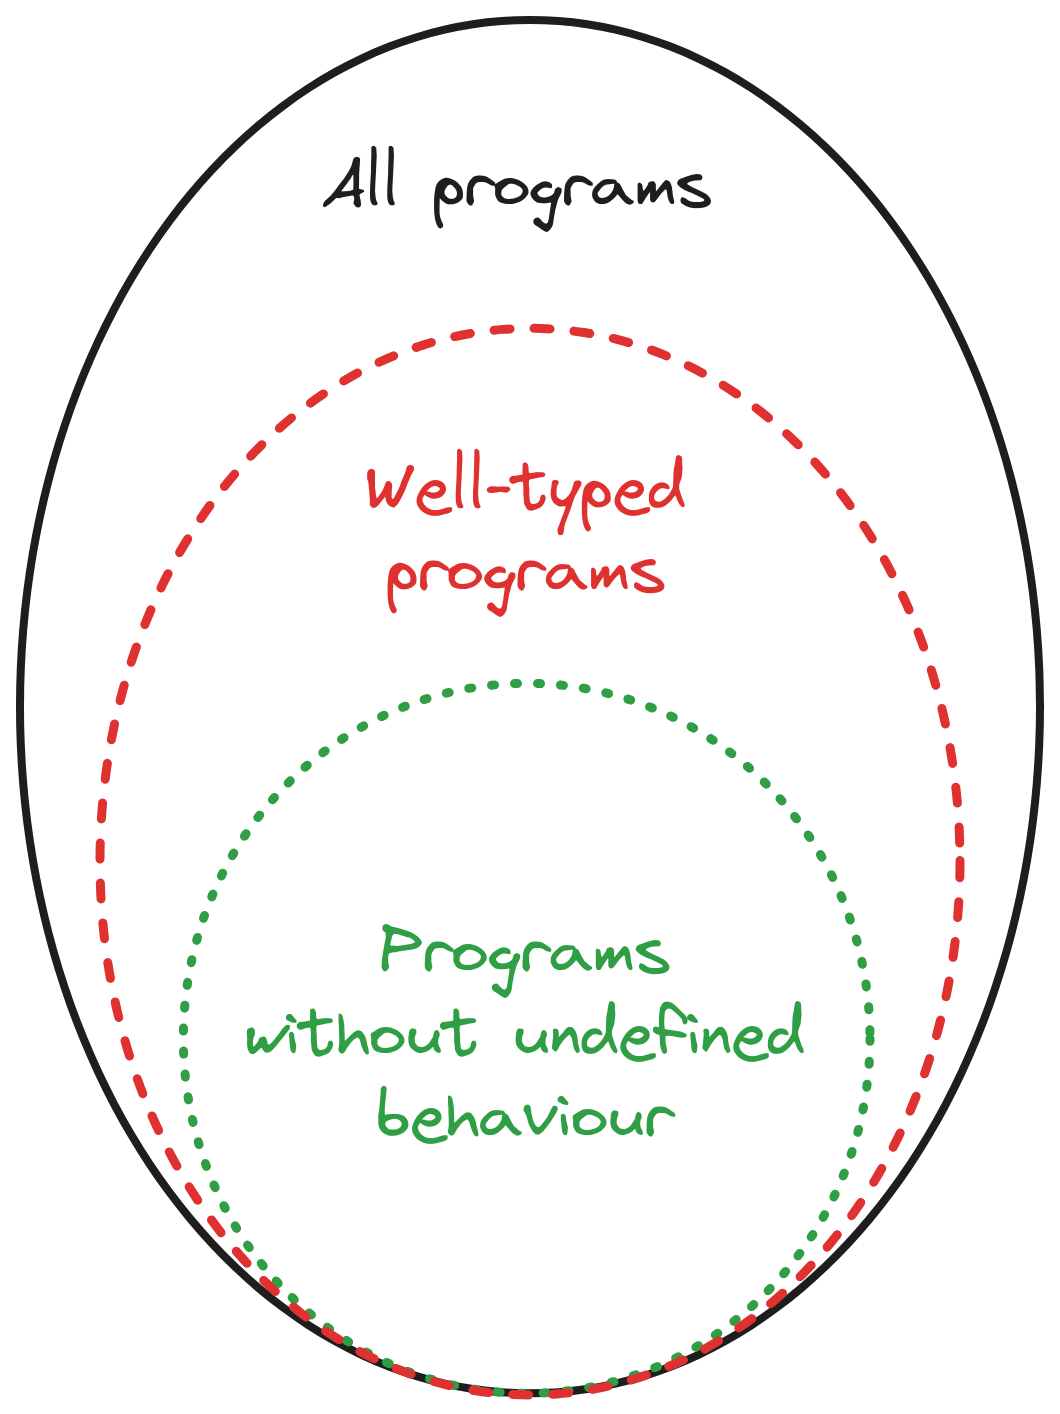
\includegraphics[width=0.5\textwidth]{images/3_translation/excalidraw_programs_venn.png}
    \caption{A diagram to show the relative powers
of increasingly restrictive program models.}
    \label{fig:excalidraw_programs_venn}
    % TODO: Check paper website for permission to reproduce
\end{figure}

When translating from languages which allow undefined behaviour such as C++ to Rust, which prohibits it my default, there are additional challenges beyond just reconciling the abstractions of the program models to express the same functionality. There are fewer safe Rust programs than C++ programs, and as a result a direct mapping to Rust may not exist if the program relies on undefined behaviour. In this case, the translation must either leverage the \mintinline{rust}{unsafe} keyword to allow such behaviour, or use a different, safe, mechanism to express the same functionality.


\subsection{Overview of HPCCG}
\label{sec:overview-hpccg}
% Overview of HPCCG

% Cite yale normally being index based
As discussed in the background to HPCCG in section \ref{ssec:hpccg}, the dominant computation kernel is an implementation of sparse matrix-vector multiplication, along with two other kernels, the vector dot product and pairwise summation of two scaled vectors. To facilitate performant implementation of these operations, HPCCG uses a non-standard, pointer based implementation of the traditionally index based Yale format to represent sparse matrices. The following example describes how HPCCG uses a pointer-based variant of the compressed row storage format to represent sparse matrices.

\begin{align}
    \begin{pmatrix}
        0 & 1 & 0 & 2 \\
        0 & 0 & 5 & 0 \\
        0 & 4 & 6 & 0 \\
        3 & 0 & 0 & 0
    \end{pmatrix}
    \label{eq:exampleMatrix}
\end{align}

A sparse matrix can then be represented as two nested lists -- one containing the non-zero values in each row, and the other the indices of those non-zero values in that row. This means the sparse matrix in (\ref{eq:exampleMatrix}) can be written as:

\begin{verbatim}
list_of_vals = [   [1, 2]  ,  [5]  ,  [4, 6]  ,  [3]   ]
list_of_inds = [   [1, 3]  ,  [2]  ,  [1, 2]  ,  [0]   ]
\end{verbatim}
% \begin{align}
%     \verb!list_of_vals = [   [1, 2]  ,  [5]  ,  [4, 6]  ,  [3]   ]! \\
%     \verb!list_of_inds = [   [1, 3]  ,  [2]  ,  [1, 2]  ,  [0]   ]!
%     \label{eq:exampleMatrixRepr}
% \end{align}

This structure uses much less memory, but has the drawback that the inner lists for each row are of variable length, making the outer list non-homogenous. HPCCG's data structure is a flattening of the above structure to use single-dimensional arrays rather than nested ones for \texttt{list\_of\_vals} and \texttt{list\_of\_inds}. This then requires a mechanism to distinguish rows, so it uses auxiliary data structures for the lengths of each row (an array of integers called \texttt{nnz\_in\_row}), along with pointers to the start of each row in the values and indices arrays (two arrays of pointers called \texttt{ptr\_to\_vals\_in\_row} and \texttt{ptr\_to\_inds\_in\_row} respectively). Finally, the number of rows (an integer called \texttt{total\_nrow}) is also needed. Hence, HPCCG would represent the sparse matrix in (\ref{eq:exampleMatrix}) as follows:

\begin{verbatim}
total_nrow          = 4
nnz_in_row          = [ 2 ,     1 , 2 ,     1 ]
list_of_vals        = [ 1 , 2 , 5 , 4 , 6 , 3 ]
ptr_to_vals_in_row  = [ ↑ ,     ↑ , ↑,      ↑ ]
list_of_inds        = [ 1 , 3 , 2 , 1 , 2 , 0 ]
ptr_to_inds_in_row  = [ ↑ ,     ↑ , ↑,      ↑ ]
\end{verbatim}

To traverse the values in a row $i$ of this data structure, first retrieve the pointer to the starting point in the list of values from \texttt{ptr\_to\_vals\_in\_row[i]}. Then, traverse through the list of values for the number of non-zeroes, \texttt{nnz\_in\_row[i]}. This same process applies to traversing indices in a row.

This data structure provides significant performance improvements over a full matrix representation for the sparse matrix-vector multiplication operation. This is because it minimises both the memory bandwidth and arithmetic operations required, by omitting the zero-values which would not contribute to the product.

Unfortunately, this pointer based implementation presents difficulties when translating to Rust, as operations on raw pointers considered unsafe, as the borrower checker is less able to reason about their memory safety. This difficulty is addressed in the first two translation versions, \ref{sec:translation-direct} and \ref{sec:translation-direct}.


\section{Implementation}
\label{sec:translation-implementation} % 3000 words

This section provides a description of the technical details of the translation process. Source code for each of these translations can be found in the \texttt{hpccg-rs} GitHub repository.
% TODO: Add process of writing incrementally optimised translations


\subsection{Direct translation}
\label{sec:translation-direct}
% Naive translation + explaining Rust ownership and borrowing
The first translation 


\subsection{Reworked data structure}
\label{sec:translation-reworked-data-structure}
% Restructured data structure

\subsection{Bounds checking}
\label{sec:translation-bounds-checking}
% Bounds checking

\subsection{Iterators}
\label{sec:translation-iterators}
% Iterators

\subsection{Shared memory parallelism}
\label{sec:translation-rayon}
% Shared-memory parallelism with Rayon

\subsection{Distributed memory parallelism}
\label{sec:translation-mpi}
% Distributed-memory parallelism with rs-mpi


\section{Equivalence checking}
\label{sec:equivalence-checking} % 3000 words

Equivalence checking is critical to make performance comparisons between programs fair. In order to draw conclusions about the performance of the Rust translation of HPCCG, there must be strong confidence that it provides the same functionality as the C++ version. Taking this to its logical extremes, a Rust program which immediately terminates will have a much lower total runtime than the C++ implementation of HPPCG, but it clearly would not be a fair comparison of Rust and C++. However, the usefulness of equivalence checking is not only for ensuring performance comparisons are fair. Any translation effort from existing C++ code to Rust 

As a result of this, a significant part of this project is developing techniques and workflows to equivalence check

\subsection{End-to-end testing}
\label{sec:equivalence-end-to-end}
% end-to-end testing

The simplest form of equivalence checking is end-to-end testing. This refers to running programs with the same input data, and asserting that they yield the same outputs.

\subsection{Formal methods}
\label{sec:equivalence-end-to-end}
% formal methods (and why they aren't suitable)

\subsection{Assembly and IR analysis}
\label{sec:equivalence-end-to-end}
% LLVM analysis (and why it is hard to scale)

\subsection{Unit testing}
\label{sec:equivalence-unit-testing}
% Unit testing

\subsubsection{Test driven development}
\label{sec:equivalence-tdd}

Test-driven development refers to


\subsection{A novel approach}
\label{sec:equivalence-polyglotest}
% polyglotest approach



% % TODO: Could omit this, it's an interesting aside, but if stuff needs to be cut, this is it
% \section{Supply-side verification}
% \label{sec:translation-supply-side-verification} % 500 words
% % Why is this important?
% % `cargo vet`


\subsection{Non-determinism in HPCCG}
\label{sec:hpccg-race-conditions}
% Explain uncommon bug resulting in non-deterministic results in HPCCG


\section{Lessons learned and proposed workflow}
\label{sec:translation-workflow} % 3000 words